%ffalse
\let\negmedspace\undefined
\let\negthickspace\undefined
\documentclass[journal,12pt,twocolumn]{IEEEtran}
\usepackage{cite}
\usepackage{amsmath,amssymb,amsfonts,amsthm}
\usepackage{algorithmic}
\usepackage{graphicx}
\usepackage{textcomp}
\usepackage{xcolor}
\usepackage{txfonts}
\usepackage{listings}
\usepackage{enumitem}
\usepackage{mathtools}
\usepackage{gensymb}
\usepackage{comment}
\usepackage[breaklinks=true]{hyperref}
\usepackage{tkz-euclide} 
\usepackage{listings}
\usepackage{gvv}                                        
%\def\inputGnumericTable{}                                 
\usepackage[latin1]{inputenc}                                
\usepackage{color}                                            
\usepackage{array}                                            
\usepackage{longtable}                                       
\usepackage{calc}                                             
\usepackage{multirow}                                         
\usepackage{hhline}                                           
\usepackage{ifthen}                                           
\usepackage{lscape}
\usepackage{tabularx}
\usepackage{array}
\usepackage{float}


\newtheorem{theorem}{Theorem}[section]
\newtheorem{problem}{Problem}
\newtheorem{proposition}{Proposition}[section]
\newtheorem{lemma}{Lemma}[section]
\newtheorem{corollary}[theorem]{Corollary}
\newtheorem{example}{Example}[section]
\newtheorem{definition}[problem]{Definition}
\newcommand{\BEQA}{\begin{eqnarray}}	
\newcommand{\EEQA}{\end{eqnarray}}
\newcommand{\define}{\stackrel{\triangle}{=}}
\theoremstyle{remark}
\newtheorem{rem}{Remark}

% Marks the beginning of the document
\begin{document}
\bibliographystyle{IEEEtran}
\vspace{3cm}

\title{18/A/E/36-49}
\author{AI24BTECH11011 - HIMANI GOURISHETTY}
\maketitle
\newpage
\bigskip

\renewcommand{\thefigure}{\theenumi}
\renewcommand{\thetable}{\theenumi}


\begin{enumerate}
	\item Let $C_1$ and $C_2$ be the graphs of the functions $y=x^2$ and $y=2x$,$0\le x\le1$ respectively.Let $C_3$ be graph of a function y=f(x),$0\le x \le 1$, f(0)=0.For a point P on $C_1$,let the lines through P,parallel to the axes, meet $C_2$and $C_3$ at Q and R respectively(see figure).If for every position of P(on $C_1$), the areas of the shaded regions OPQ and ORP are equal, determine the function of f(x).
\hfill{(1998-8 Marks)}
\begin{figure}[h!]
\centering
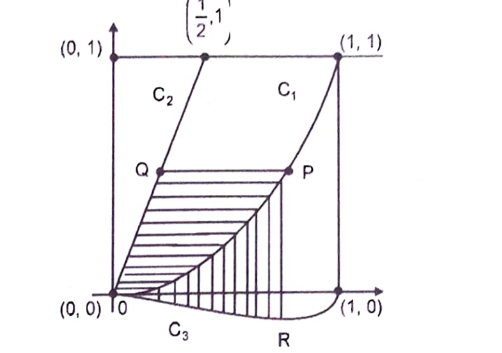
\includegraphics[width=1\linewidth]{figs/fig1.png}
\label{fig:11011}
\end{figure}
				        
\item Integrate $\int_{0}^{\pi}\frac{e^{cosx}}{e^{cosx}+e^{-cosx}}$
\hfill{(1999-2 Marks)}\\	             
							      
							      \item Let f(x) be a continuos function given by \\

f(x)=
							
$\begin{cases}

2x,& |x|\le1\\
x^2+ax+b,&|x|>1

\end{cases}$
							

							
\item Find the area of the region in the third quadrant bounded by the curves x=-2$y^2$ and y=f(x) lying on the left of the line $8x+1$=0.  
							
\hfill{(1999-10marks)}\\
														    
							      \item For $x > 0 $,$let f(x)=\int_{e}^{x}\frac{lnt}{1+t}$.Find the function$ f(x) + f(\frac{1}{x})$
and show that $f(e)+f(\frac{1}{e})=
\frac{1}{2}$ .Here ,lnt=log t.
							

\hfill{(2000-5Marks)}
															    \item Let $b\neq0$ and for j=0,1,2,...,n, $S_j$ be the area of the region bounded by the y-axis and the curve $xe^{ay}$ = sin by $\frac{jr}{b} \le y \le \frac{(j+1)\pi}{b}$ .Show that  $S_0,S_1,S_2,......,S_n$ are in geometric progression . Also , find their sum for a=-1and b=$pi$.\\.
															      \hfill{(2001-5Marks)}
					

\item Find the area of the region bounded by the curves $y=x^2$ ,$y=|2-x|$ and $y=2$, which lies to the right of the line $x=1$.
								\hfill{(2002-5 Marks)}
							       \item If f is an even function then prove that 																	 
$\int_{0}^{\frac{\pi}{2}}f(cos2x)cox $ =$\sqrt{2}\int_{0}^{\frac{\pi}{4}}f(sin2x)cosx$\\												
\hfill{(2003-2Marks)}
																	        
							      \item If $y(x)=\int_{\frac{\pi^2}{16}}^{x^2}\frac{cosxcos\sqrt{\theta}}{1+sin^2\sqrt{\theta}}$, then find $\frac{dy}{dx}$ at x=$pi$\\.
								\hfill{(2004-2Marks)}

							      \item  Find the value of $\int_{\frac{-\pi}{3}}^{\frac{\pi}{3}}\frac{\pi+4x^3}{2-cos(|x|+\frac{\pi}{3})}$\\.
								\hfill{(2004-4Marks)}
								\item	Evaluate $\int_{0}^{\pi}e^{cosx}(2sin(\frac{1}{2}cosx)+3cos(\frac{1}{2}cosx))sinx$\\.
								\hfill{(2005-2Marks)}
							      \item Find the area bounded by the curves \\  
$x^2=y,x^2=-y$ and $y^2=4x-3$
																						          \hfill{(2005-4Marks)}
																							  \item  f(x) is a differentiable function and g(x) is  double differentiable function such that $f(x)|\le1$ and f'(x)=g(x). if $f^2(0)+g^2(0)$=9. Prove that there exist some $c\in(-3,3)$ such that $g(c).g"(c)<0$.\\.
								\hfill{(2005-6Marks)}

						        	\item 
  \[
\begin{bmatrix}
4a^2 & 4a & 1\\
4b^2 & 4b & 1\\						      4c^2 & 4c & 1\\
\end{bmatrix}
\begin{bmatrix}
f(-1)\\
f(1)\\
f(2)
																														         \end{bmatrix}
																															    =
																															\begin{bmatrix}
3a^2+3a\\						
3b^2+3b\\
3c^2+3c
\end{bmatrix}
\]
f(x) is a quadratic function and its maximum value occurs at a point V.A is a point of intersection of y=f(x) with x axis and point B is such that chord AB subtends a right angle at V . Find the area enclosed by f(x) and chord AB.
\hfill{(2005-6Marks)}
\item The value of 5050 $\frac{\int_{0}^{1}(1-x^50)^100}{\int{0}^{1} {(1-x^50)^101}}$
\hfill{(2006-6M)}


\end{enumerate}


\end{document}
